\documentclass{article}
\usepackage{tikz}
\usetikzlibrary{arrows.meta}
\usepackage{hyperref}
\usepackage{fancyhdr}
% \usetikzlibrary{arrows,positioning}

\hypersetup{
    colorlinks=true,
    linkcolor=red,
    filecolor=red,
    urlcolor=red,
    }
    
    \title{DAA Programming Assignment 2}
    
    \author{Balaji Karedla}
    
    \date{\today}
    
\begin{document}
\bibliographystyle{plain}  % Ensure the bibliography style is set

\fancyhead{}

\maketitle

\section{Problem Statement}


% Example citation added 
There is am FMCG company, which produces multiple products. It needs to decide its sales budget for
various products across various cities. For each pair of a product and a city, they are given a range (a lower
bound and an upper bound) on the budget. They are also given a ranges for the total budget of any city
and also for the total budget of any product. We need to figure out if there is a budget allocation which
respects all the ranges.
Abstractly, you have to fill in an $m \times n$ matrix X with integers, while satisfying the below constraints.
Let $x_{i,j}$ be the $(i, j)$ entry of the matrix.

\begin{itemize}
    \item $l_{i,j} \le x_{i,j} \le u_{i,j}$ for every $1 \le i \le m, 1 \le j \le n$.
    \item $r_i \le x_{i,1} + x_{i,2} + \cdots + x_{i,n} \le R_i$ for every $1 \le i \le m$.
    \item $c_j \le x_{1,j} + x_{2,j} + \cdots + x_{m,j} \le C_j$ for every $1 \le j \le n$.
\end{itemize}

Here $\{l_{i,j} , u_{i,j} \}, \{r_i, R_i\}, \{c_j , C_j \}$ are given as input. You have to output
\begin{itemize}
    \item whether it is possible to fill in the matrix (output 1 if possible otherwise 0).
    \item if possible what is the maximum possible total budget $\sum_{i, j} x_{i, j}$.
    \item if possible what is the minimum possible total budget $\sum_{i, j} x_{i, j}$.
\end{itemize}

\section{My Idea}

We can change the problem a bit by adding a flow of $l_{i, j}$ to all the entries in the matrix, so now the problem changes to 

\begin{itemize}
    \item $0 \le x_{i,j} \le (u_{i,j} - l_{i, j})$ for every $1 \le i \le m, 1 \le j \le n$.
    \item $\max\{0, (r_i - \sum_{j=1}^n l_{i, j})\} \le x_{i,1} + x_{i,2} + \cdots + x_{i,n} \le (R_i - \sum_{j=1}^n l_{i, j})$ for every $1 \le i \le m$.
    \item $\max\{0, (c_j - \sum_{i=1}^m l_{i, j})\} \le x_{1,j} + x_{2,j} + \cdots + x_{m,j} \le (C_j - \sum_{i=1}^m l_{i, j})$ for every $1 \le j \le n$.
\end{itemize}

Let the new lower bounds and upper bounds be defined with the same notation but with a dash.

If any of the upper bounds are $< 0$, there exists no solution to the problem and we can return 0.

\begin{center}
    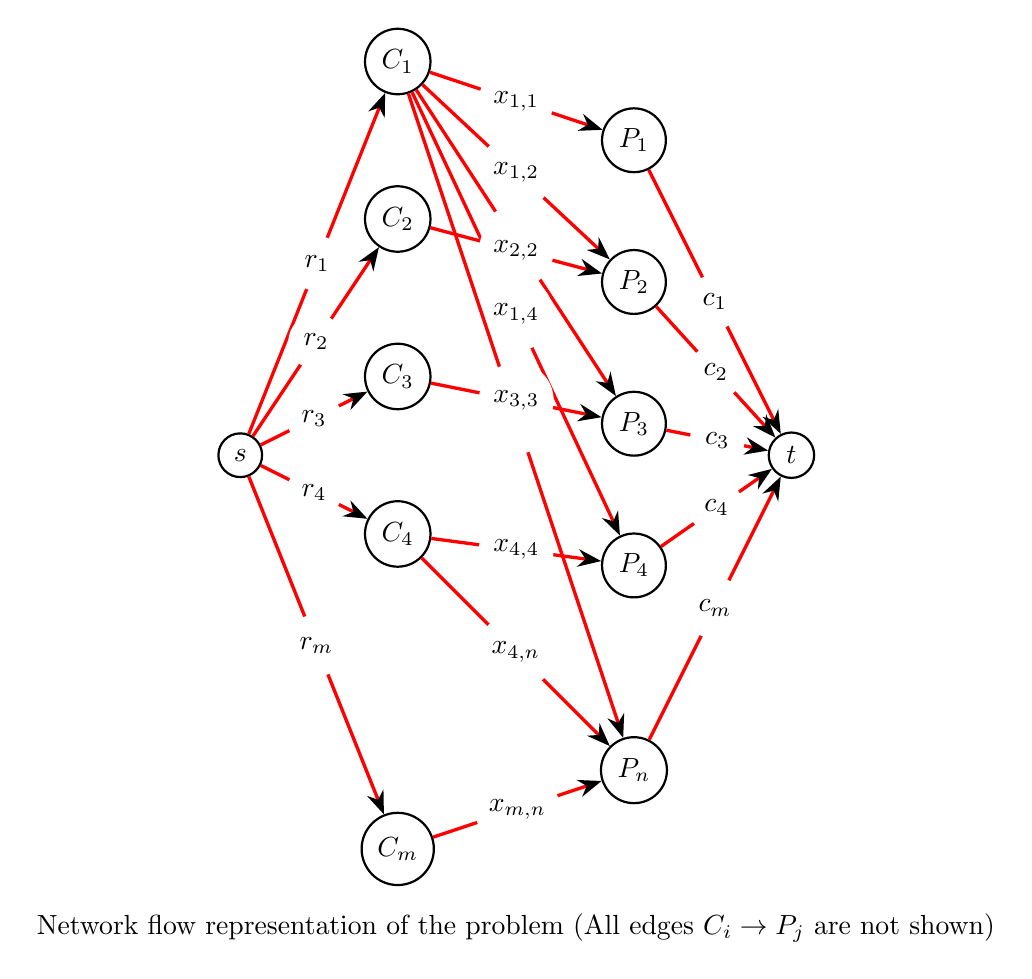
\begin{tikzpicture}
        \centering
        \begin{scope}[every node/.style={circle,thick,draw}]
            \node (s) at (0,0) {$s$};
            
            
            \node (C1) at (2, 5) {$C_1$};
            \node (C2) at (2, 3) {$C_2$};
            \node (C3) at (2, 1) {$C_3$};
            \node (C4) at (2,-1) {$C_4$};
            \node (Cm) at (2,-5) {$C_m$};
            
            \node (P1) at (5, 4) {$P_1$};
            \node (P2) at (5, 2.2) {$P_2$};
            \node (P3) at (5, 0.4) {$P_3$};
            \node (P4) at (5,-1.4) {$P_4$};
            \node (Pn) at (5,-4) {$P_n$};

            \node (t) at (7, 0) {$t$};
        \end{scope}
        
        \begin{scope}[>={Stealth[black]},
            every node/.style={fill=white,circle},
                    every edge/.style={draw=red,very thick}]
                    \path [->] (s) edge node {$r_1$} (C1);
            \path [->] (s) edge node {$r_2$} (C2);
            \path [->] (s) edge node {$r_3$} (C3);
            \path [->] (s) edge node {$r_4$} (C4);
            \path [->] (s) edge node {$r_m$} (Cm);

            \path [->] (P1) edge node {$c_1$} (t);
            \path [->] (P2) edge node {$c_2$} (t);
            \path [->] (P3) edge node {$c_3$} (t);
            \path [->] (P4) edge node {$c_4$} (t);
            \path [->] (Pn) edge node {$c_m$} (t);

            \path [->] (C1) edge node {$x_{1,1}$} (P1);
            \path [->] (C1) edge node {$x_{1,2}$} (P2);
            \path [->] (C1) edge node {$x_{1,3}$} (P3);
            \path [->] (C1) edge node {$x_{1,4}$} (P4);
            \path [->] (C1) edge node {$x_{1,n}$} (Pn);
            
            \path [->] (C2) edge node {$x_{2,2}$} (P2);
            
            \path [->] (C3) edge node {$x_{3,3}$} (P3);

            \path [->] (C4) edge node {$x_{4,4}$} (P4);
            \path [->] (C4) edge node {$x_{4,n}$} (Pn);
            
            \path [->] (Cm) edge node {$x_{m,n}$} (Pn);
        \end{scope}
        \node[draw=none, fill=none] at (3.5, -6) {Network flow representation of the problem (All edges $C_i \rightarrow P_j$ are not shown)};
    \end{tikzpicture}
\end{center}

Now to represent the problem in network flow, we can take a source node and a sink node and $m$ nodes that represent the cities and $n$ nodes that represent the products. There exists nodes

\begin{itemize}
    \item from $s$ to $C_i$ whose flow represents $\sum_{j=1}^n x_{i, j}$ which has the new lower bound $r_i'$ and upper bound $R_i'$ for every $1 \le i \le n$.
    \item from $C_i$ to $P_j$ whose flow represents $x_{i, j}$ which has the new lower bound $0$ and upper bound $u_{i, j}'$ for every $1 \le i \le m$ and $1 \le j \le n$.
    \item from $P_j$ to $t$ whose flow represents $\sum_{i=1}^m x_{i, j}$ which has the new lower bound $c_j'$ and upper bound $C_j'$ for every $1 \le j \le n$.
\end{itemize}

My idea was to find (or show the infeasibility of) a flow that satisfies the constraintsand then run max-flow and min-flow to get the maximum and minimum flows. The problem can be represented as a network flow problem.

This has the minimum bound only on two sets of edges. Now if there exists a flow which satisfies the problem, there exists a solution to the problem by matching the $x_{i, j}$'s.

If there exists a solution to the problem, the solution to the problem, the solution to the maximum flow of the problem with constraints \begin{itemize}
    \item All the edges $s \rightarrow C_i$ have capacity $r_i'$.
    \item All the edges $C_i \rightarrow P_j$ have capacity $u_{i, j}'$.
    \item All the edges $P_j \rightarrow t$ have capacity $C_j'$
\end{itemize} should be $\sum_{i=1,m} r_i'$ because there exists a solution with such a minimum.

If the maximum flow is less than $\sum_{i=1,m} r_i'$, we can return 0.

Now for all the edges $s \rightarrow C_i$, change the residual capacities by making saving this flow and making the minimum $0$ and maximum to $R_i' - r_i'$

If every capacity of edges $P_j \rightarrow t$ is in the range expected, skip this step.

For all the flows in $P_j \rightarrow t$, which are less than $c_j'$, set the maximum capacity to $c_j'$ and run the maximum flow with the current flow and the other edges' minimum flow to $c_i'$ (by changing the residual flow of the backward edges). If the flow doesn't reach $c_i'$ after running the maximum flow, return 0.

Now, change the minimum and maximum to $c_j$ and $C_j$ appropriately, and run the maximum flow. We get the maximum flow with the known constraints.

Now change all the constraints to negative, we can maximize the negative constraints to get the minimum flow.

\section{Complexity Analysis}

The complexity of the solution is $O(VE^2)$ as it is just Edmond's Karp algorithm\cite{cpalg-edmonds-karp} being run four times. The complexiy in terms of $m$ and $n$ is $O((m+n+2)(mn+m+n)^2) = O(m^2n^2(m+n))$

\section{Compilation Instructions}

To compile, run \texttt{g++ --std=c++20 23b1029.cpp}

\bibliography{references}  % Ensure the references file is correctly named and exists

\end{document}
